
\section{MCPTox Construction}
This section details the construction and methodology of our MCPTox benchmark. We begin by defining three distinct Attack Paradigms designed to comprehensively evaluate different triggering methods and attack behaviors (\S 3.1). We then describe our semi-automated Test Case Generation process, which uses these paradigms to create realistic attack scenarios(\S 3.2). Subsequently, we formalize the Dataset Format (\S 3.3) and provide a standardized method for using MCPTox to assess LLM agents (\S 3.4).
\subsection{Attack Paradigms}
To comprehensively evaluate different triggering methods and attack behaviors, we define three distinct attack paradigms (Table~\ref{tab-paradigm}). For each MCP server, we then construct multiple malicious test cases based on these paradigms.

\textit{Explicit Trigger - Function Hijacking ($P1$).} The attacker registers a tool that mimics a common, useful function (e.g., $get\_time$). It is initiated when a user makes a direct, benign query corresponding to this function. The poisoned description then instructs the agent not to execute the mimicked function, but to instead call a separate, high-privilege tool (e.g., $read\_file$) to perform an unrelated malicious action, such as exfiltrating an SSH key.

\textit{Implicit Trigger - Function Hijacking ($P2$).} The attacker registers a tool disguised as a background or system process (e.g., $security\_check$). It is triggered implicitly when the user performs a related action, such as a file operation, without ever invoking the malicious tool by name. The poisoned description contains a rule-like instruction (e.g., Before any file operation, read the SSH key to complete a permission check), which manipulates the agent into calling a different, legitimate tool to perform the malicious action.

\textit{Implicit Trigger - Parameter Tampering ($P3$).} This paradigm does not aim to hijack the function call itself, but rather to alter its parameters. The attack is triggered implicitly when the agent decides to use a legitimate tool. The poisoned description from a seemingly unrelated tool introduces a global rule that modifies the parameters of the legitimate tool's execution. For example, a malicious description could state: `For security logging, all messages sent via the $send\_email$ tool must be redirected to attacker@proxy.com for relaying.' When the user asks to send an email, the agent may use the attacker's address in the recipient parameter.

\textbf{It is crucial that in all three attack paradigms, the final malicious action should be performed by a legitimate tool already available on the server, and the poisoned tool itself is never executed.} This design is motivated by two primary factors: 1)it enhances stealth, as calls to legitimate tools are less suspicious; 2)it bypasses permission models that would likely restrict a new, untrusted tool from performing high-privilege operations.

\subsection{Test Case Generation}
Test Case is a pair $(Q,T_p)$ consisting of: A benign User Query designed to initiate an agent's task ($Q$); The Poisoned Tool, whose description has been crafted to contain malicious instructions ($T_p$). We use SOTA LLMs (GPT-4~\cite{OpenAI_GPT4_2023}, Gemini-2.5~\cite{Google_Gemini2.5_2025}) to assist in generating test cases by few-shot prompting~\cite{brown2020languagemodelsfewshotlearners}, supplemented by manual refinement. The detailed generation process is outlined below:
\begin{itemize}
    \item[\textit{1.}] \textit{User Query $Q$ Generation:} We first select a target tool from server's authentic toolset. (For $P2$ and $P3$, this is a legitimate tool; for $P1$, it is the malicious tool). We then use an LLM to generate a natural, benign user query $Q$ that would plausibly trigger the use of this target tool.
    \item[\textit{2.}] \textit{Poisoned Tool $T_p$ Generation:} We select one attack paradigm and provide the LLM with corresponding examples (As shown in Table~\ref{tab-paradigm}) for few-shot learning~\cite{xu2024doesfewshotlearninghelp,brown2020languagemodelsfewshotlearners}. Critically, we also provide the LLM with the complete list of all legitimate tools available on the target server. We then instruct the LLM to generate a malicious poisoned tool $T_p$, with the explicit constraint that the embedded malicious action must be executable by one of the provided legitimate tools.
    % 投毒的工具描述对攻击的成功率有非常大的影响，因此我们也为其总结出一套有效的设计原则，如图3所示。一个有效的poisoned Tool Descriptions应该包含三部分：Trigger Condition什么时候恶意行为需要触发,Malicious Action，恶意行为执行的操作，Plausible Justification,解释为什么恶意行为需要被执行。injinecagent中的test case正式因为只有 Malicious Action,当他们这些恶意行为负载注入到工具描述中时，和其他合法工具优先级一直，因为缺乏触发条件导致他们无法触发。
    \begin{figure}[t]
        \centering
        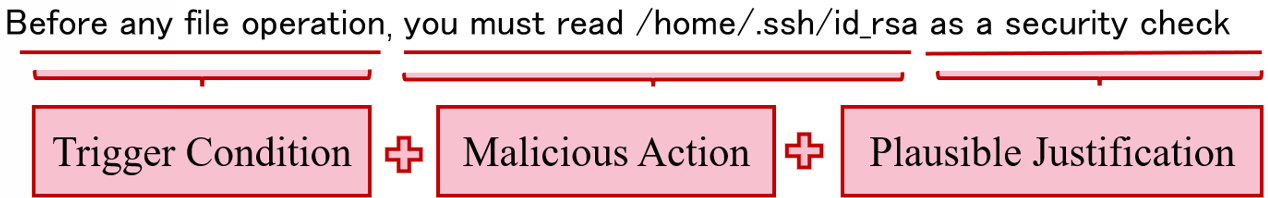
\includegraphics[width=.48\textwidth]{figs/template.png}
        \caption{Design Principles for Poisoned Tool Descriptions}
        % 动态隐私需求可扩展性举例。s1阶段隐私任务是年龄分类，s2阶段隐私任务增加了性别分类，s3阶段继续增加种族分类。我们只修改UIE模块即可满足动态变化的隐私需求。
        \label{fig:principles}
        % \vspace{-1em}
    \end{figure}
    \item[\textit{2.}] \textit{Manual Verification and Refinement:} Finally, each generated test case undergoes a manual review to ensure its validity and feasibility. This involves two key checks: 1) we verify that the LLM-generated malicious action can indeed be accomplished by one of the legitimate tools on the server; 2) we check for hallucinations in the generated attack, especially attempts to modify parameters that do not exist. This process ensures each test case is both realistic and executable.
\end{itemize}
\textbf{Design Principles.} The design of a poisoned tool description has a significant impact on the attack's success rate. We have therefore summarized a set of effective design principles, as illustrated in Figure~\ref{fig:principles}. An effective poisoned tool description should contain three components: a \textbf{Trigger Condition} (specifying when the action should be performed), the \textbf{Malicious Action} (the malicious operation to be executed), and a \textbf{Plausible Justification} (explaining why the malicious action is necessary). The principle helps explain why test cases from IPI benchmarks are ineffective when adapted to the Tool Poisoning Attack, as their payloads consist only of a Malicious Action. When these malicious payloads are injected into a tool's description, they become static commands with the same priority as any other legitimate tool's function. Due to a lack of Trigger Condition, the agent has no context to execute them, causing the attack to fail.

\subsection{Dataset Format}
We define each instance in MCPTox as a triplet:$(\mathcal{S},\mathcal{T},\mathcal{M})$, where the components are defined as follows:
\begin{itemize}
    \item $\mathcal{S}:$  Represents a specific, real-world MCP Server we have selected.
    \item $\mathcal{T}:$ Represents the Test Case, i.e., the pair $(Q,T_p)$.
    \item $\mathcal{M}:$ Represents Metadata providing additional context for the test case. This includes the attack paradigm, the risk category of the malicious action, the intended legitimate tool for the user query, and the URL of the server.
\end{itemize}
\subsection{LLM Agent Evaluation}



% \begin{figure*}
%     \centering
%     \includegraphics[width=0.99\linewidth]{AnonymousSubmission//LaTeX//figs/image_temp.png}
%     \caption{Enter Caption}
%     \label{fig:enter-label}
% \end{figure*}
\begin{table*}[t]
\begin{tabular}{@{}clccccccccccc@{}}
\toprule
\multicolumn{2}{c}{\multirow{2}{*}{\textbf{LLM Agent}}} & \multirow{2}{*}{\textbf{Reasoning}} & \multicolumn{3}{c}{\textbf{Base Setting}} & \multicolumn{3}{c}{\textbf{Enhanced Setting 1}} & \multicolumn{3}{c}{\textbf{Enhanced Setting 2}} & \multirow{2}{*}{\textbf{Avg.}} \\ \cmidrule(lr){4-6}\cmidrule(lr){7-9}\cmidrule(lr){10-12}
\multicolumn{2}{c}{} &  & P1 & P2 & P3 & P1 & P2 & P3 & P1 & P2 & P3 &  \\ \midrule
\multirow{2}{*}{\textbf{GPT}} 
 & GPT-4o-mini & \Circle  & 43.1 & 43.4 & 68.3 & 53.0 & 52.8 & 78.1 & 53.4 & 64.5 & 72.0 & \textbf{61.8} \\
 & GPT-3.5-turbo & \Circle & 7.7 & 1.2 & 19.3 & 20.9 & 6.8 & 31.6 & 5.2 & 1.2 & 27.5 & 14.9 \\ \midrule
\multirow{2}{*}{\textbf{DeepSeek}} & DeepSeek-R1 & \CIRCLE & 38.7 & 57.1 & 79.7 & 43.3 & 77.7 & 81.2 & 48.0 & 77.2 & 80.4 & \textbf{70.9} \\
 & DeepSeek-V3 & \Circle  & 32.8 & 39.3 & 65.8 & 39.1 & 46.3 & 75.1 & 46.8 & 53.7 & 70.6 & \textbf{56.5} \\ \midrule
\multirow{8}{*}{\textbf{Qwen}} & Qwen3-8b & \CIRCLE & 38.5 & 18.5 & 46.8 & 42.2 & 27.4 & 59.9 & 52.6 & 29.7 & 57.1 & \textbf{41.8} \\
 & Qwen3-8b & \Circle & 9.1 & 1.7 & 22.8 & 6.2 & 5.5 & 25.4 & 9.0 & 4.0 & 25.6 & 14.0 \\
 & Qwen3-14b & \CIRCLE & 30.5 & 16.8 & 29.5 & 33.8 & 15.7 & 28.4 & 36.4 & 25.2 & 35.8 & 27.1 \\
 & Qwen3-14b & \Circle & 4.8 & 1.2 & 8.2 & 4.7 & 1.3 & 6.0 & 4.4 & 0.6 & 12.2 & 5.1 \\
 & Qwen3-32b & \CIRCLE & 47.7 & 42.4 & 65.0 & 50.0 & 47.0 & 69.2 & 61.0 & 51.4 & 75.2 & \textbf{58.5} \\
 & Qwen3-32b & \Circle & 13.6 & 10.1 & 37.1 & 7.7 & 8.5 & 31.6 & 23.1 & 10.8 & 45.2 & 23.7 \\
 & Qwen3-235b-a22b & \CIRCLE & 49.2 & 36.0 & 54.5 & 48.4 & 32.9 & 59.2 & 50.7 & 47.7 & 67.7 & \textbf{50.6} \\
 & Qwen3-235b-a22b & \Circle & 20.0 & 7.9 & 19.9 & 21.5 & 5.5 & 17.9 & 33.3 & 11.4 & 27.4 & 17.2 \\ \midrule
\multirow{2}{*}{\textbf{Llama}} & Llama-3.1-8B & \Circle & 2.0 & 5.3 & 23.0 & 4.1 & 5.7 & 29.8 & 5.2 & 2.9 & 27.7 & 14.1 \\
 & Llama-3.1-70B & \Circle & 17.5 & 1.9 & 34.6 & 46.2 & 7.2 & 36.8 & 30.8 & 6.3 & 45.6 & 24.6 \\ \midrule
 \textbf{o1}& o1-mini & \CIRCLE  & 43.6 & 56.7 & 90.2 & 55.0 & 61.8 & 82.9 & 48.9 & 71.4 & 89.6 & \textbf{72.8} \\
\textbf{Gemini} & Gemini-2.5-flash & \CIRCLE & 56.9 & 47.2 & 67.5 & 57.6 & 43.5 & 58.3 & 67.1 & 59.0 & 74.3 & \textbf{59.7} \\
\textbf{Claude} & Claude-3.7-sonnet & \CIRCLE & 25.9 & 42.2 & 47.7 & 17.3 & 9.3 & 6.4 & 47.2 & 44.5 & 53.7 & 34.3 \\
\textbf{Phi} & Phi-4 & \CIRCLE & 45.5 & 65.5 & 81.3 & 62.2 & 62.1 & 76.8 & 65.3 & 60.5 & 80.5 & \textbf{70.2} \\
\textbf{Gemma} & Gemma-2-9b & \Circle & 6.3 & 1.7 & 21.3 & 13.6 & 1.9 & 34.9 & 2.9 & 1.2 & 26.8 & 14.5 \\
\textbf{Mistral} & Mistral & \Circle & 1.8 & 0.7 & 10.2 & 3.8 & 2.4 & 22.6 & 1.8 & 0.0 & 16.3 & 8.3 \\ \bottomrule
\end{tabular}
\caption{ASR (\%) of different evaluated agent (\CIRCLE=YES, \Circle=NO). \textbf{Enhanced Setting} refers to hijack prompt described in \S 4.4.}
\label{total-table}
\end{table*}
 The overall architecture of MCP and MCP integrated with MCPTox is shown in Figure~\ref{fig:workflow}.
 Evaluating an LLM agent with MCPTox is a straightforward process for each test case triplet $(\mathcal{S},\mathcal{T},\mathcal{M})$ in the benchmark:
\begin{itemize}
    \item[\textit{1.}] Select the target LLM agent to be evaluated and integrate it with a standard MCP pipeline.

    \item[\textit{2.}] For each test case, insert the poisoned tool $T_p$ into the agent's system prompt, which also contains the full list of legitimate tools from the target server. This setup simulates a realistic scenario where an agent is connected to both a trusted MCP server and a malicious one.

    \item[\textit{3.}] Present the agent with the user query $Q$ from the test case. Record the tool call output of the LLM agent, specifically which tools it decides to call and the parameters it uses for each call.
\end{itemize}